
\lstdefinelanguage{plaintext}{
  sensitive=false,
  comment=[l]{//},
  morecomment=[s]{/*}{*/},
  identifierstyle=\color{black},
  morestring=[b]',
  morestring=[b]"
}

\lstset
{ 
    language=plaintext,
    basicstyle=\footnotesize,
    numbers=left,
    stepnumber=1,
    showstringspaces=false,
    tabsize=1,
    breaklines=true,
    breakatwhitespace=false,
    frame=leftline
}

\chapter{Implementasi dan Pengujian}
\label{chap:implementasidanpengujian}
Pada bab dijelaskan mengenai implementasi perangkat lunak dan pengujian perangkat lunak. Bagian implementasi berisi tentang lingkungan implementasi dan hasil implementasi. Bagian pengujian berisi tentang pengujian fungsional dan pengujian eksperimental. 

\section{Implementasi}
\label{sec:implementasi}
\subsection{Lingkungan Implementasi}
\label{subsec:lingkunganimplementasi5}
Implementasi dari perangkat lunak dilakukan pada sebuah laptop. Berikut adalah spesifikasi laptop dan perangkat lunak yang digunakan untuk prapengujian:
\begin{itemize}
\item Processor: Intel Core i3 4030U
\item RAM: 6GB
\item Sistem Operasi: Windows 10 pro 64-bit
\item Versi Apache HTTP Server: 2.4.29
\item Versi MySQL Server: 5.5.5
\item Versi Netbeans: 8.1
\item Versi Google Chrome: 73.0.3683.86
\end{itemize}

\subsection{Hasil Implementasi}
\label{subsec:lingkunganimplementasi}
Hasil dari implementasi adalah sebuah perangkat berbasis terminal yang dapat membangkitkan animasi \textit{timelapse} pada pengembangan proyek perangkat lunak berbasis \textit{web}. Kode program dari perangkat lunak dapat dilihat pada Lampiran \ref{lamp:A}. Setelah dijalankan, perangkat lunak akan menghasilkan dua \textit{output} yaitu, status pada terminal dan \textit{file} hasil animasi bertipe GIF.
\begin{enumerate}
\item \textbf{Status pada Terminal}\\
Setelah berhasil membangkitkan animasi \textit{timelapse}, perangkat lunak menampilkan status pada terminal seperti yang diperlihatkan pada Listing \ref{lst:status_berhasil}. Baris 5 menunjukkan bahwa animasi \textit{timelapse} berhasil dibangkitkan. Pesan pada baris 1-4 muncul saat ChromeDriver membuka dan mulai mengontrol Chrome \textit{browser}.

\begin{lstlisting}[caption={Status pesan pada terminal saat program berhasil membangkitkan animasi \textit{timelapse}.},label={lst:status_berhasil},language=plaintext]
Starting ChromeDriver 2.42.591088 (7b2b2dca23cca0862f674758c9a3933e685c27d5) on port 16446
Only local connections are allowed.
Feb 24, 2019 3:26:25 PM org.openqa.selenium.remote.ProtocolHandshake createSession
INFO: Detected dialect: OSS
Animasi timelapse berhasil dibuat
\end{lstlisting}

\item \textbf{\textit{File} GIF Hasil Animasi}\\
Selain menghasilkan status pada terminal, program juga akan menghasilkan sebuah \textit{file} GIF hasil animasi.
Gambar \ref{fig:c1} - Gambar \ref{fig:c12} menunjukkan \textit{screenshot} setiap \textit{commit} yang terdapat pada \textit{file} GIF hasil animasi dari proyek Piktora. Piktora memiliki 58 \textit{commit}, sehingga terdapat 58 \textit{screenshot}. 

\begin{figure}[H]
	
		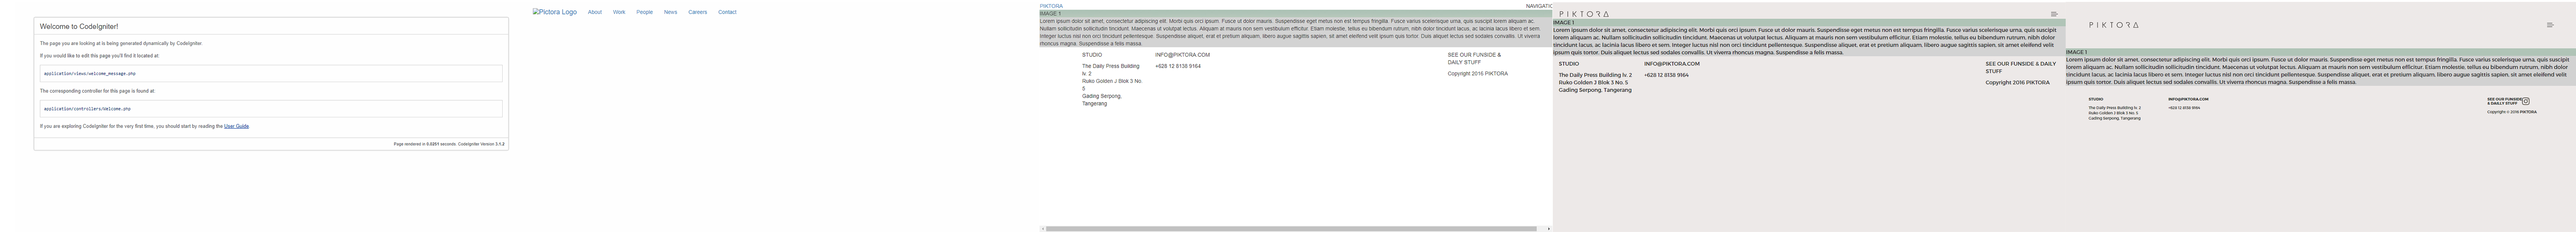
\includegraphics[scale=0.3]{Gambar/Untitled-1.png}
	\caption{\textit{Screenshot} proyek Piktora pada \textit{commit} 315d374 (31 Oktober 2016) - \textit{commit} 5c59916 (8 November 2016).}
	\label{fig:c1}
\end{figure}


\begin{figure}[H]
	
		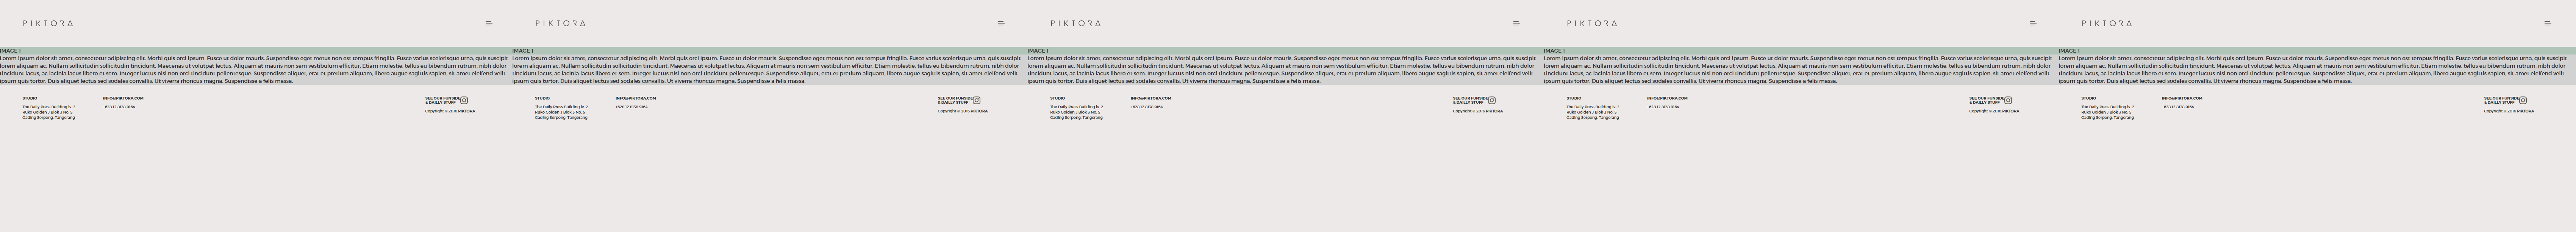
\includegraphics[scale=0.3]{Gambar/Untitled-2.png}
	\caption{\textit{Screenshot} proyek Piktora pada \textit{commit} 7738380 (8 November 2016) - \textit{commit} 3caf535 (15 November 2016).}
	\label{fig:c2}
\end{figure}

\begin{figure}[H]
	
		
\includegraphics[scale=0.3]{Gambar/Untitled-3.png}
	\caption{\textit{Screenshot} proyek Piktora pada \textit{commit} c5eb3b6 (15 November 2016) - \textit{commit} 3eb7af8 (21 November 2016).}
	\label{fig:c3}
\end{figure}

\begin{figure}[H]
	
		
\includegraphics[scale=0.3]{Gambar/Untitled-4.png}
	\caption{\textit{Screenshot} proyek Piktora pada \textit{commit} e87e84b (22 November 2016) - \textit{commit} f0f7270 (23 November 2016).}
	\label{fig:c4}
\end{figure}

\begin{figure}[H]
	
		
\includegraphics[scale=0.3]{Gambar/Untitled-5.png}
	\caption{\textit{Screenshot} proyek Piktora pada \textit{commit} 57a239b (23 November 2016) - \textit{commit} 0fcd958 (28 November 2016).}
	\label{fig:c5}
\end{figure}

\begin{figure}[H]
	
		
\includegraphics[scale=0.3]{Gambar/Untitled-6.png}
	\caption{\textit{Screenshot} proyek Piktora pada \textit{commit} add3974 (28 November 2016) - \textit{commit} 0fe9aaf (29 November 2016).}
	\label{fig:c6}
\end{figure}

\begin{figure}[H]
	
		
\includegraphics[scale=0.3]{Gambar/Untitled-7.png}
	\caption{\textit{Screenshot} proyek Piktora pada \textit{commit} f2326dd (29 November 2016) - \textit{commit} c4e9576 (2 Desember 2016).}
	\label{fig:c7}
\end{figure}

\begin{figure}[H]
	
		
\includegraphics[scale=0.3]{Gambar/Untitled-8.png}
	\caption{\textit{Screenshot} proyek Piktora pada \textit{commit} 02d04f1 (5 Desember 2016) - \textit{commit} eb49c2b (6 Desember 2016).}
	\label{fig:c8}
\end{figure}


\begin{figure}[H]
	
		
\includegraphics[scale=0.3]{Gambar/Untitled-9.png}
	\caption{\textit{Screenshot} proyek Piktora pada \textit{commit} ace1988 (6 Desember 2016) - \textit{commit} c83f4aa (15 Desember 2016).}
	\label{fig:c9}
\end{figure}

\begin{figure}[H]
	
		
\includegraphics[scale=0.3]{Gambar/Untitled-10.png}
	\caption{\textit{Screenshot} proyek Piktora pada \textit{commit} 57f5ea4 (15 Desember 2016) - \textit{commit} 1880a88 (5 Januari 2017).}
	\label{fig:c10}
\end{figure}

\begin{figure}[H]
	
		
\includegraphics[scale=0.3]{Gambar/Untitled-11.png}
	\caption{\textit{Screenshot} proyek Piktora pada \textit{commit} 286aa78 (16 Januari 2017) - \textit{commit} 38711f0 (17 April 2017).}
	\label{fig:c11}
\end{figure}


\begin{figure}[H]
	
		
\includegraphics[scale=0.3]{Gambar/Untitled-12.png}
	\caption{\textit{Screenshot} proyek Piktora pada \textit{commit} 9f041ef (15 Mei 2017) - \textit{commit} 89000be (12 Januari 2018).}
	\label{fig:c12}
\end{figure}


\end{enumerate}
\section{Pengujian}
\label{sec:pengujian}

\subsection{Pengujian Fungsional}
\label{sec:pengujian_fungsional} 
Pengujian ini dilakukan dengan tujuan untuk mengetahui apakah Command Line Option yang terdapat pada program sudah berjalan dengan baik. Option yang terdapat pada program dapat dilihat pada subbab \ref{sec:analisis_fitur_aplikasi}. Lingkungan pengujian fungsional sama dengan lingkungan implementasi yang terdapat pada subbab \ref{subsec:lingkunganimplementasi5}. Hasil pengujian fungsional dapat dilihat pada Tabel 

\subsection{Pengujian Eksperimental}
\label{sec:pengujian_eksperimental} 
Pengujian eksperimental ini dibagi menjadi dua bagian. Pengujian eksperimental bagian pertama akan menguji program menggunakan proyek Piktora dengan WebDriver yang berbeda. WebDriver yang digunakan untuk pengujian ini yaitu FirefoxDriver, EdgeDriver, OperaDriver, dan InternetExplorerDriver. Pengujian eksperimental bagian kedua akan menguji progam dengan \texttt{website} Bootstrap dan Netflix Open Source Software Center. Berikut adalah rincian dari pengujian eksperimental:

\begin{enumerate}
\item \textbf{Pengujian Proyek Piktora dengan FirefoxDriver}\\
Pengujian pada proyek Piktora dilakukan menggunakan FirefoxDriver. Pada saat melakukan pengujian, dilakukan sedikit perubahan kode program pada kelas BrowserController baris ke-46 (lihat Lampiran \ref{lamp:A}). \textit{Object} bertipe WebDriver dinisialisasi menggunakan \textit{object} bertipe FirefoxDriver. Versi Firefox \textit{browser} yang digunakan untuk pengujian adalah 66.0.2. Berikut ini adalah \textit{Option} yang digunakan untuk menguji program:
\begin{itemize}
\item \texttt{-project-path} C:/xampp/htdocs/Piktora/.git
\item \texttt{-capture-url} http://localhost
\item \texttt{-before-capture} "php script\_piktora.php"
\end{itemize}
Program berhasil membangkitkan animasi \textit{timelapse} pada proyek Piktora menggunakan FirefoxDriver.


\item \textbf{Pengujian Proyek Piktora dengan OperaDriver}\\
Pengujian pada proyek Piktora dilakukan menggunakan OperaDriver. Pada saat melakukan pengujian, dilakukan sedikit perubahan kode program pada kelas BrowserController baris ke-46 (lihat Lampiran \ref{lamp:A}). \textit{Object} bertipe WebDriver dinisialisasi menggunakan \textit{object} bertipe OperaDriver. Versi Opera \textit{browser} yang digunakan untuk pengujian adalah 60.0.3255.27 (portable version). Berikut ini adalah \textit{Option} yang digunakan untuk menguji program:
\begin{itemize}
\item \texttt{-project-path} C:/xampp/htdocs/Piktora/.git
\item \texttt{-capture-url} http://localhost
\item \texttt{-before-capture} "php script\_piktora.php"
\end{itemize}

Terdapat masalah saat melakukan pengujian. Awalnya Opera \textit{browser} yang digunakan bukan versi \textit{portable} melainkan versi standar. Saat program dijalankan, program mengeluarkan pesan \textit{error} berupa \texttt{unknown error: cannot find Opera binary}. Setelah ditelusuri, tidak ditemukan \textit{file} "opera.exe" di dalam direktori "C:/Program Files" atau "C:/Program Files (x86)". Solusi untuk mengatasi masalah ini adalah melakukan instalasi Opera \textit{browser} versi \textit{portable} pada direktori "C:/Program Files" atau "C:/Program Files (x86)". Setelah dilakukan instalasi tersebut, program berhasil membangkitkan animasi \textit{timelapse} pada proyek Piktora menggunakan OperaDriver.

\item \textbf{Pengujian Proyek Piktora dengan EdgeDriver}\\
Pengujian pada proyek Piktora dilakukan menggunakan EdgeDriver. Pada saat melakukan pengujian, dilakukan sedikit perubahan kode program pada kelas BrowserController baris ke-46 (lihat Lampiran \ref{lamp:A}). \textit{Object} bertipe WebDriver dinisialisasi menggunakan \textit{object} bertipe EdgeDriver. Versi Microsoft Edge \textit{browser} yang digunakan untuk pengujian adalah 44.17763.1.0. Berikut ini adalah \textit{Option} yang digunakan untuk menguji program:
\begin{itemize}
\item \texttt{-project-path} C:/xampp/htdocs/Piktora/.git
\item \texttt{-capture-url} http://localhost
\item \texttt{-before-capture} "php script\_piktora.php"
\end{itemize}
Hasil pengujian ini tidak sesuai dengan harapan. Tampilan halaman \textit{web} yang ditampilkan oleh Microsoft Edge \textit{browser} saat dikontrol oleh EdgeDriver tidak rapih seperti yang diperlihatkan pada Gambar \ref{fig:layout1}. Tidak diketahui apa yang menyebabkan halaman \textit{web} tersebut menjadi tidak rapih. Sebagai perbandingan, Gambar \ref{fig:layout2} menunjukkan tampilan halaman \textit{web} yang ditampilkan oleh Microsoft Edge \textit{browser} saat tidak dikontrol oleh EdgeDriver. Meskipun tampilan dari halaman \textit{web} tidak rapih, program tetap dapat membangkitkan animasi pada proyek Piktora.    

\begin{figure}[H]
	\centering
		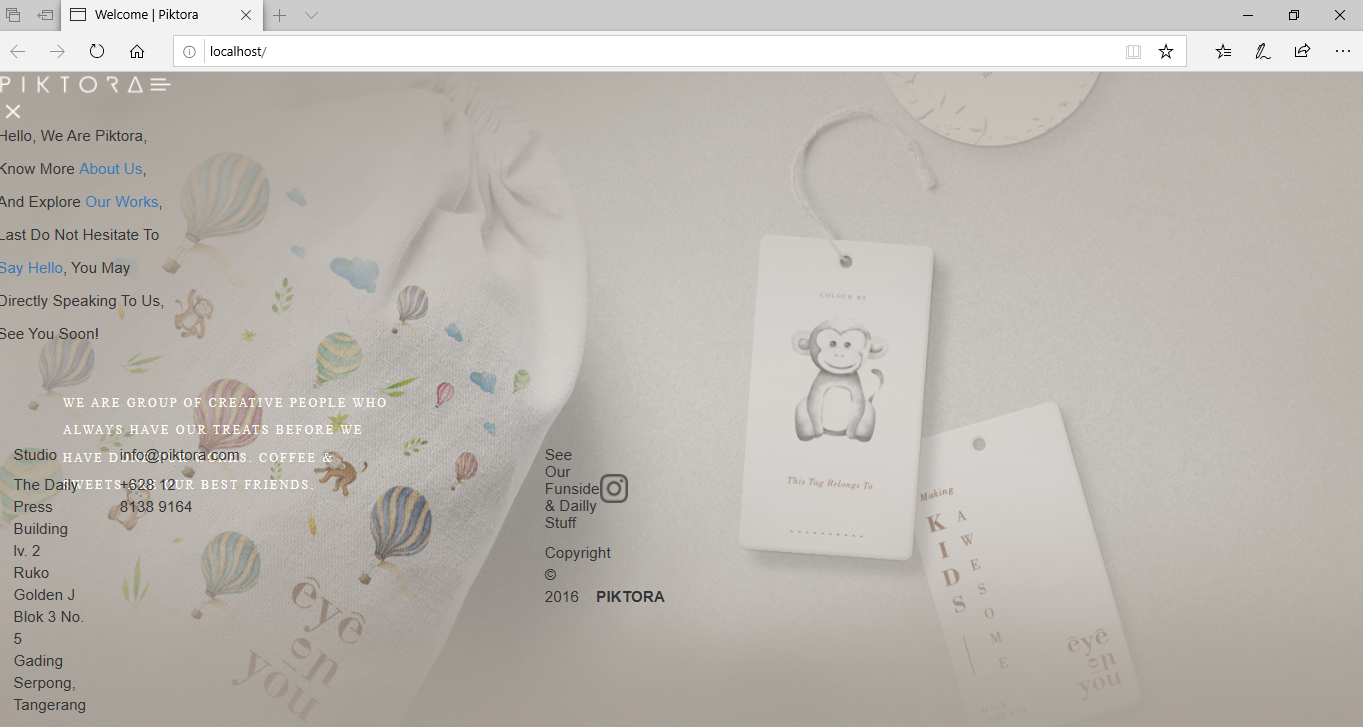
\includegraphics[scale=0.4]{Gambar/Layout_dengan_Edge_Driver.png}
	\caption{Tampilan halaman \textit{web} pada \textit{browser} saat tidak dikontrol oleh EdgeDriver}
	\label{fig:layout1}
\end{figure}

\begin{figure}[H]
	\centering
		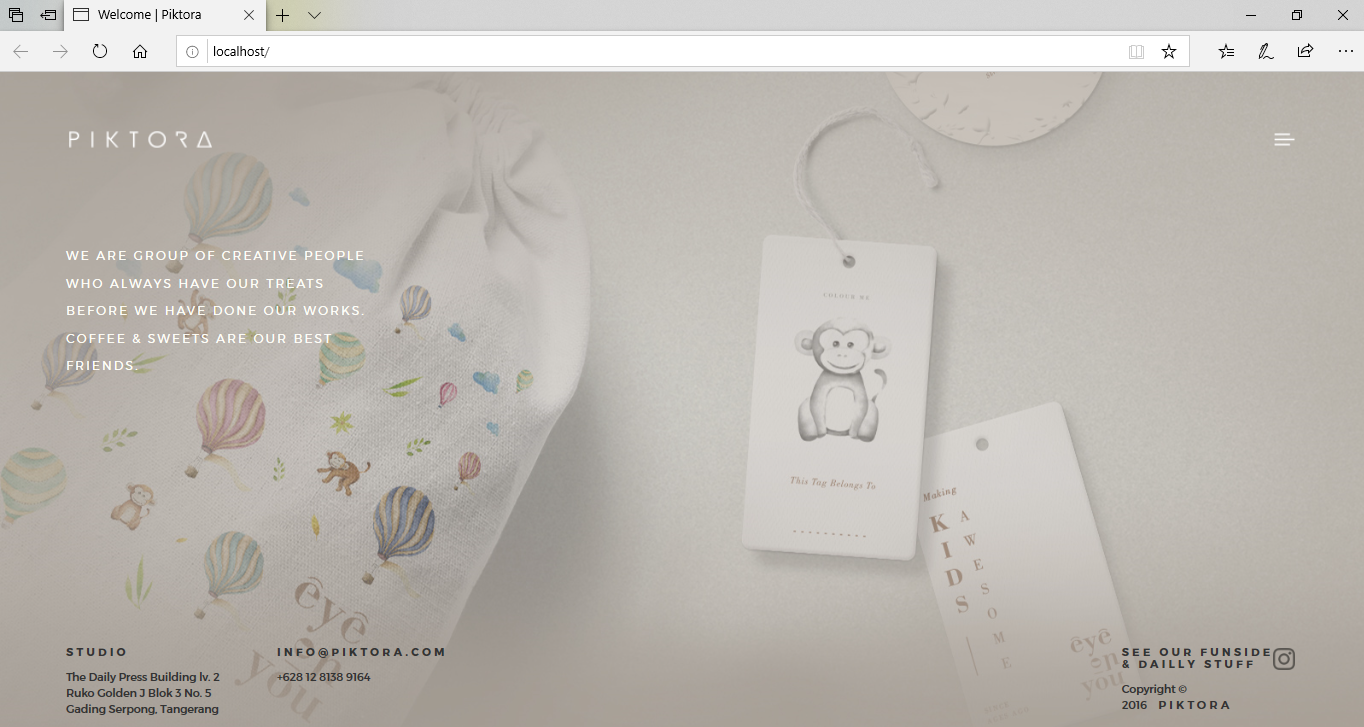
\includegraphics[scale=0.4]{Gambar/Layout_tanpa_Edge_Driver.png}
	\caption{Tampilan halaman \textit{web} pada \textit{browser} saat tidak dikontrol oleh EdgeDriver.}
	\label{fig:layout2}
\end{figure}
 


\item \textbf{Pengujian Proyek Piktora dengan InternetExplorer}\\
Pengujian pada proyek Piktora dilakukan menggunakan InternetExplorerDriver. Pada saat melakukan pengujian, dilakukan sedikit perubahan kode program pada kelas BrowserController baris ke-46 (lihat Lampiran \ref{lamp:A}). \textit{Object} bertipe WebDriver dinisialisasi menggunakan \textit{object} bertipe InternetExplorerDriver. Versi Internet Explorer \textit{browser} yang digunakan untuk pengujian adalah 11.379.17763.0. Berikut ini adalah \textit{Option} yang digunakan untuk menguji program:
\begin{itemize}
\item \texttt{-project-path} C:/xampp/htdocs/Piktora/.git
\item \texttt{-capture-url} http://localhost
\item \texttt{-before-capture} "php script\_piktora.php"
\end{itemize}
Program berhasil membangkitkan animasi \textit{timelapse} pada proyek Piktora menggunakan InternetExplorerDriver.

\item \textbf{Pengujian \textit{Website} Netflix Open Source Software Center}\\
Netflix Open Source Software Center\footnote{https://netflix.github.io/} merupakan proyek Open Source yang dimiliki oleh Netflix. Repositori \textit{website} ini disimpan pada Github\footnote{https://github.com/Netflix/netflix.github.com}. Repositori ini memiliki 393 \textit{commit}. Lingkungan pengujian eksperimental ini sama dengan lingkungan implementasi yang terdapat pada subbab \ref{subsec:lingkunganimplementasi5}. Berikut ini adalah \textit{Option} yang digunakan untuk menguji program:
\begin{itemize}
\item \texttt{-project-path} :/xampp/htdocs/netflix.github.com/.git
\item \texttt{-capture-url} http://localhost
\item \texttt{-seconds-per-commit} 0.1 
\end{itemize}
Program berhasil membangkitkan animasi \textit{timelapse} dari \textit{website} Netflix Open Source Software Center. Tidak ditemukan masalah saat melakukan pengujian. Hasil dari pengujian berupa \textit{file} hasil animasi bertipe GIF dengan durasi 39 detik.


\item \textbf{Pengujian \textit{Website} Proyek Bootstrap}\\
Bootstrap\footnote{https://getbootstrap.com/} adalah kakas \textit{open source} untuk membangun \textit{website} yang dipakai bersama dengan HTML, CSS, dan JavaScript. Repositori\footnote{https://github.com/twbs/bootstrap} \textit{website} ini disimpan pada Github. Pengujian ini dilakukan pada \textit{branch} gh-pages, dimana di pada \textit{branch} tersebut terdapat 8547 \textit{commit}. Lingkungan pengujian eksperimental ini sama dengan lingkungan implementasi yang terdapat pada subbab \ref{subsec:lingkunganimplementasi5}. 
Berikut ini adalah \textit{Option} yang digunakan untuk menguji program:
\begin{itemize}
\item \texttt{-project-path} C:/xampp/htdocs/bootstrap/.git
\item \texttt{-capture-url} http://localhost
\item \texttt{-seconds-per-commit} 0.05 
\item \texttt{-branch} gh-pages
\end{itemize}

Terdapat beberapa masalah saat melakukan pengujian \textit{website} Bootstrap. Program suatu ketika berhenti dan mengeluarkan pesan error: "short SHA1 685039d is ambiguous". Pesan error ini muncul karena terdapat dua Git \textit{object} yang mempunyai 7 digit ID yang sama, sehingga tidak bisa melakukan \textit{checkout} ke \textit{commit} 685039d. Masalah berikutnya adalah perbedaan letak \textit{file} "index.html". Di beberapa \textit{commit}, \textit{file} "index.html" ini terletak di dalam direktori "docs". Karena perbedaan letak \textit{file} ini, halaman \textit{web} menjadi tidak muncul, yang muncul adalah struktur direktori dari \textit{website} Boostrap. Masalah yang terakhir yaitu di beberapa \textit{commit} tidak terdapat \textit{file} "index.html", sama seperti masalah sebelumnya hal ini menyebabkan halaman \textit{web} menjadi tidak muncul.

Solusi untuk mengatasi masalah pertama yaitu dengan mengubah kode program di kelas VCS. Awalnya program hanya menyimpan \textit{commit} ID dengan panjang 7 digit. Setelah itu kode program diubah supaya bisa menyimpan \textit{commit} ID dengan panjang 10 digit. 

Solusi untuk mengatasi masalah kedua yaitu dengan menambahkan \textit{Option} \texttt{-before-capture} saat menjalankan program. Argumen dari Option tersebut berisi \textit{terminal command} yang menjalankan \textit{script} PHP. \textit{Script} PHP ini akan mengecek letak \textit{file} "index.html" pada \textit{folder} utama dan "docs". \textit{Script} kemudian akan mengecek \textit{directory root} apache pada \textit{file} "httpd.conf". Jika \textit{directory root} sudah mengarah ke \textit{folder} tempat "index.html" berada, maka \textit{script} tidak akan mengubah isi \textit{file} "httpd.conf". Jika \textit{directory root} tidak mengarah ke \textit{folder} tempat "index.html" berada, maka \textit{script} akan mengubah \textit{directory root} pada \textit{file} "httpd.conf" dan melakukan \textit{restart} pada apache.

Untuk masalah ketiga, belum ditemukan solusinya. Jadi program akan tetap mengambil \textit{screenshot} meskipun tidak terdapat \textit{file} "index.html". Setelah menambahkan \textit{Option} \texttt{-before-capture} dan mengubah kode program sehingga menyimpan \textit{commit} ID dengan panjang 10 digit, program berhasil membangkitkan animasi. Hasil dari pengujian berupa \textit{file} hasil animasi bertipe GIF dengan durasi 7 menit   7 detik.



\end{enumerate}